\documentclass[a4]{beamer}
\usepackage{amssymb}
\usepackage{graphicx}
\usepackage{subfigure}
\usepackage{newlfont}
\usepackage{amsmath,amsthm,amsfonts}
%\usepackage{beamerthemesplit}
\usepackage{pgf,pgfarrows,pgfnodes,pgfautomata,pgfheaps,pgfshade}
\usepackage{mathptmx}  % Font Family
\usepackage{helvet}   % Font Family
\usepackage{color}

\mode<presentation> {
 \usetheme{Default} % was Frankfurt
 \useinnertheme{rounded}
 \useoutertheme{infolines}
 \usefonttheme{serif}
 %\usecolortheme{wolverine}
% \usecolortheme{rose}
\usefonttheme{structurebold}
}

\setbeamercovered{dynamic}

\title[MA4413]{Statistics for Computing \\ {\normalsize MA4413 Lecture 3A}}
\author[Kevin O'Brien]{Kevin O'Brien \\ {\scriptsize Kevin.obrien@ul.ie}}
\date{Autumn Semester 2013}
\institute[Maths \& Stats]{Dept. of Mathematics \& Statistics, \\ University \textit{of} Limerick}

\renewcommand{\arraystretch}{1.5}

\begin{document}

\begin{frame}
\titlepage
\end{frame}

%---------------------------------------------------------------------------%
\frame{
\frametitle{Today's Class}
\large
\begin{itemize}
\item More on Graphical methods
\begin{itemize}
\item Bar charts
\item Box-and-whisker plots
\end{itemize}
\item Discrete probability distributions
\begin{itemize}
\item Binomial Experiments
\item The Binomial Probability distribution
\end{itemize}
\end{itemize}
}
%------------------------------------------------------------------%
\frame{
\frametitle{Bar plots}
\large
\begin{itemize} \item A bar plot displays the frequency (or relative frequency) for all observations of a discrete random variable. \item A bar plot is much like a histogram, in that the heights of columns represent the frequency (or relative frequency) of each outcome.
\item Each outcome of a random experiment corresponds to one and only one column of the bar plot.
\item A bar plot differs from a histogram in that the columns are distinct and separated from each other by a small distance.
\end{itemize}
}
%------------------------------------------------------------------%
\frame{
\frametitle{Bar plots}
\large
Suppose we roll a die 300 times, and obtain the following results

\begin{center}
\begin{tabular}{|c|c|c|c|c|c|c|}
  \hline

  Outcome & 1 & 2 & 3 & 4 & 5 & 6 \\
  Frequency & 59 &41 &39 &52 &57 &52  \\
  Rel. Freq & 0.196 & 0.136 & 0.130 & 0.173 & 0.190 & 0.173\\
  \hline
\end{tabular}
\end{center}

On the next slide is the bar plot of the relative frequencies of the outcomes of die throw experiment.
Included on the bar plot is the theoretical probability of each outcome. As each outcome is equally probable, this is just a straight line.\\ \bigskip
Minor deviations from the theoretical probability can often be assumed to be as a result of random error. In the case of large deviations, there may be a flawed assumption about the theoretical probabilities.
}

%--------------------------------------------------------%

\frame{
\frametitle{Relative Frequency Bar Plots}

\begin{center}
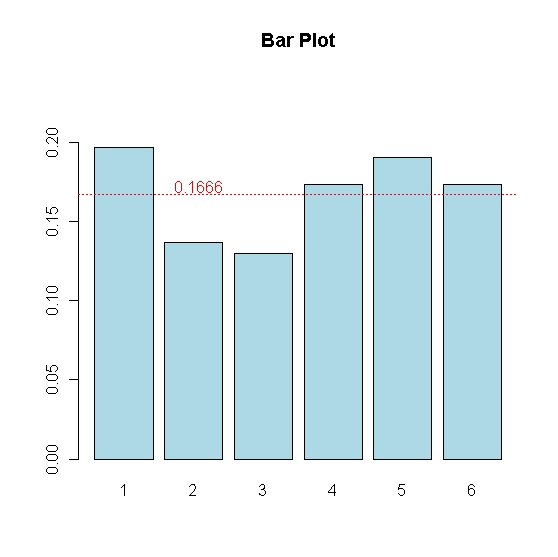
\includegraphics[scale=0.40]{3Bbarplot}
\end{center}
}

%--------------------------------------------------------%

\frame{
\frametitle{Relative Frequency Bar Plots}

\begin{itemize}
\item Just as bar plots can be used to graphically depict observed relative frequencies, they can be used to
depict the theoretical probabilities of each outcome.
\item We will be using bar plots to visualize the theoretical probabilities of outcomes of discrete random variables.
\item For this module, bar plots are assumed to be used for this purpose, unless it is clearly expressed otherwise.
    \item On the next slide is a bar plot of the probabilities of each outcome of a dice throw.
\end{itemize}

}


%--------------------------------------------------------%

\frame{
\frametitle{Bar Plots}
\begin{center}
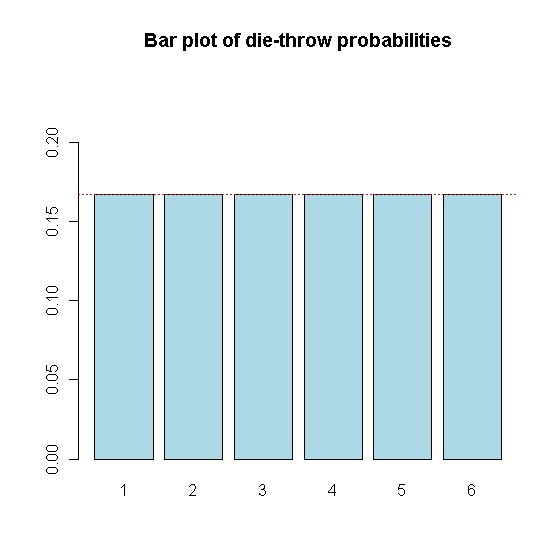
\includegraphics[scale=0.40]{3Bbarplot3}
\end{center}
}

\frame{
\frametitle{Bar Plots}

\begin{itemize}
\item Bar plots are useful in that they visualize `events'.
\item Consider the event where either a `4' or a `5' is thrown.
\item The relevant columns for this event are shaded (next slide).
\item We will be using bar plots for depicting specific events in upcoming material
\end{itemize}

}
%--------------------------------------------------------%

\frame{
\frametitle{Bar Plots}

\begin{center}
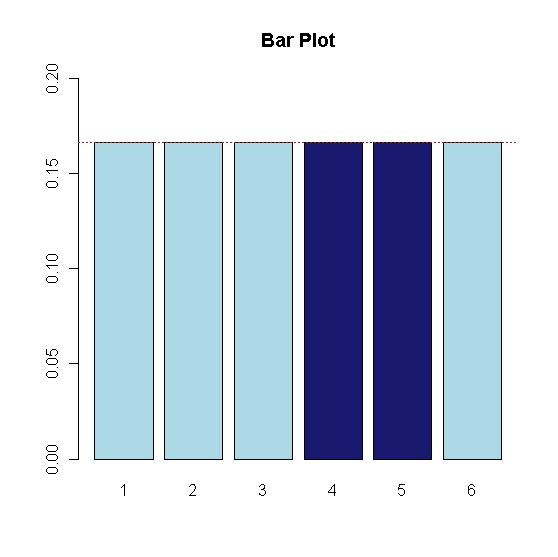
\includegraphics[scale=0.40]{3Bbarplot2}
\end{center}
}


%---------------------------------------------------------------------------%

\frame{
\frametitle{Boxplots}
\begin{itemize}
\item The second graphical method we will be looking at today is the `box-and-whisker' plot (commonly just referred to as `boxplots')
\item The boxplots is a useful tool for assessing the distribution of a dataset, by means of a visual summary.
\item Recall the data set of the exam scores of 100 students from yesterday's class (see next slide).
\item The quartiles of the data set were $Q_1 = 42.5$, $Q_2 = 54.5$ (with $Q_2$ being the median), and $Q_3 =  65.5$ respectively.
\item The interquartile range is $Q_3 - Q_1 = 23$
\item The boxplot of the distribution is featured on the next slide.
\end{itemize}
}
%---------------------------------------------------------------------------%
\frame{
\begin{table}[ht]
\caption{Exam results of 100 students} % title of Table
\centering % used for centering table
\begin{tabular}{|c ccc ccc ccc|} % centered columns (4 columns)\hline
\hline

13	&	21	&	22	&	23	&	24	&	25	&	26	&	28	&	29	&	30	\\	31	&	32	&	33	&	34	&	35	&	 36	&	36	&	36	&	37	&	38	\\
39	&	41	&	41	&	41	&	42	&	43	&	44	&	44	&	44	&	45	\\	45	&	46	&	47	&	49	&	50	&	 51	&	51	&	52	&	53	&	53	\\
53	&	53	&	53	&	54	&	54	&	54	&	54	&	54	&	54	&	54	\\	55	&	55	&	55	&	56	&	56	&	 56	&	57	&	57	&	58	&	59	\\
62	&	63	&	63	&	63	&	63	&	64	&	64	&	64	&	64	&	64	\\	65	&	65	&	65	&	65	&	65	&	 66	&	66	&	66	&	67	&	69	\\
71	&	71	&	72	&	72	&	73	&	74	&	75	&	76	&	76	&	76	\\	77	&	82	&	84	&	85	&	87	&	 88	&	91	&	91	&	92	&	99	\\ \hline
\end{tabular}
\end{table}
}
%--------------------------------------------------------%

\frame{
\frametitle{Boxplots}

\begin{center}
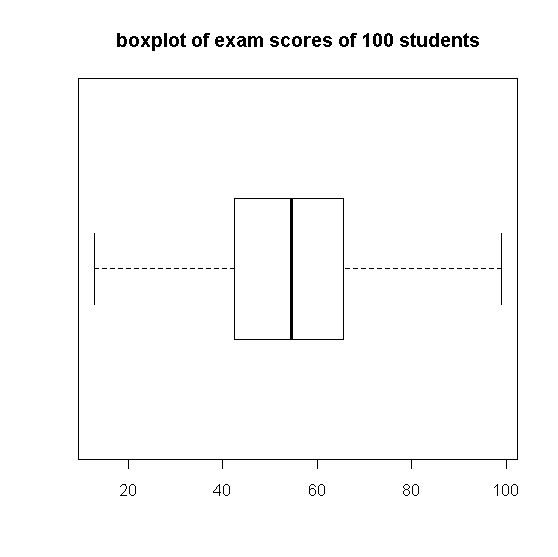
\includegraphics[scale=0.40]{3Bboxplot1}
\end{center}
}

%--------------------------------------------------------%
\frame{
\frametitle{Boxplots}
\begin{itemize}
\item The boxplot is a visual summary containing important aspects of a distribution. \item The main component of the plot , the `\textbf{\emph{box}}', stretches from the \textbf{\emph{lower hinge}}, defined as $Q_1$, to the \textbf{\emph{upperhinge}}, defined as $Q_3$ .
\item The median is shown as a line across the box.
\item Therefore the box contains the middle half of the scores in the distribution.
\item  1/4 of the distribution is between the median line and the upper hinge. Similary 1/4 of the distribution is between the median line and the lower hinge.
\end{itemize}
}
%---------------------------------------------------------------------------%
\frame{
\frametitle{Boxplots}
\begin{itemize}
\item On either side of the box are the \textbf{\emph{whiskers}}.
\item To find where to place the whiskers, we must first compute the location of the \textbf{\emph{fences}}, and determine whether or not there are any \textbf{\emph{outliers}} present.
\item Firstly, we must compute the location of the \textbf{\emph{lower fence}}.
\[ \mbox{ Lower Fence}  = Q_1 - 1.5 \times IQR \]
\item For our example, the lower fence is
\[ \mbox{ Lower Fence}  = 42.5 - 1.5 \times 23  = 42.5 - 34.5 = 8 \]

\end{itemize}
}
%---------------------------------------------------------------------------%
\frame{
\frametitle{Boxplots}
\begin{itemize}
\item The lower fence is used to determine whether there are any outliers in the lower half of the data set.
\item If there is any observed value less than the lower fence, it is considered an outlier.
\item The first whisker is drawn at the location of the lowest value that is not considered an outlier.
\item If no values are considered outliers, then the whisker is drawn at the location of the smallest value of the dataset.
\item For our dataset, the lowest value is 13, which is not less than the lower fence.
\item Therefore we draw the first whisker , a vertical line, at this location.
\item A horizontal line is drawn connecting the location of this whisker to $Q_1$.
\end{itemize}
}
\frame{
\frametitle{Boxplots}
\begin{itemize}
\item Any value considered to be an outlier should be indicated with an asterisk or a small circle.
\item We will see an example of a boxplot with outliers in due course.
\end{itemize}


}
%---------------------------------------------------------------------------%
\frame{
\frametitle{Boxplots}
\begin{itemize}
\item Now we must compute the location of the \textbf{\emph{upper fence}}.
\[ \mbox{ Upper Fence}  = Q_3 + 1.5 \times IQR \]
\item For our example, the upper fence is
\[ \mbox{ Upper Fence}  = 65.5  + 1.5 \times 23  = 65.5 + 34.5 = 100 \]

\end{itemize}
}
%---------------------------------------------------------------------------%
\frame{
\frametitle{Boxplots}
\begin{itemize}
\item The upper fence is used to determine whether there are any outliers in the upper half of the data set.
\item If there is any observed value greater than the upper fence, it is considered an outlier.
\item The second whisker is drawn at the location of the highest value that is not considered an outlier.
\item If no values are considered outliers, then the whisker is drawn at the location of the highest value of the dataset.
\item For our dataset, the highest value is 99, which is less than the upper fence.
\item Therefore we draw the second whisker , a vertical line, at this location.
\item A horizontal line is drawn connecting the location of this whisker to $Q_3$.
\end{itemize}
}
%---------------------------------------------------------------------------%
\frame{
\frametitle{Boxplots}
\begin{itemize}
\item Remark: If you do not get a sensible value for either the upper or lower fence, you can replace it with the nearest sensible value
\item For example, suppose we got a negative lower fence value. It does not make sense to get a negative score in an exam.
\item In this case, we could replace the value with a value of $0$.
\item similarly for the upper fence: any fence value greater than 100 should be replaced with the value of 100.
\end{itemize}
}
%---------------------------------------------------------------------------%
\frame{
\frametitle{Boxplots}
\begin{itemize}
\item Boxplots are very useful in comparing the distributions of two or more data sets.
\item Recall the experiment of 60 students, each throwing a die 100 times.
\item Suppose they perform this experiment twice, firstly with a fair die, and then with a crooked die.
\item (The probability of the outcomes from the crooked die are as per yesterday's class).
\item Boxplots can use used to compare the distribution of the outcomes of both experiments.
\end{itemize}
}

%--------------------------------------------------------%

\frame{
\frametitle{Boxplots}

\begin{center}
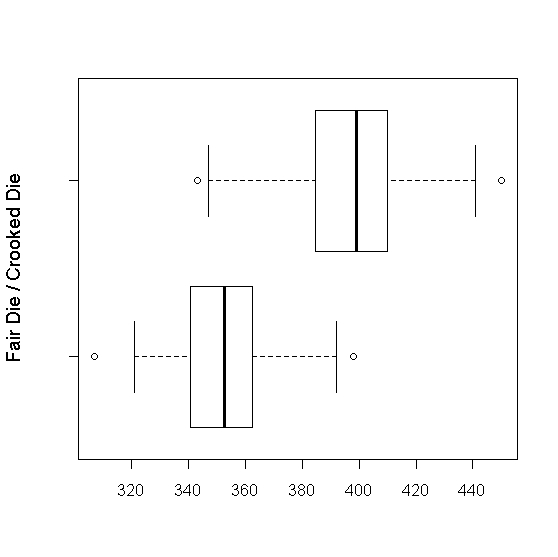
\includegraphics[scale=0.40]{3Bboxplot2}
\end{center}
}

%--------------------------------------------------------------------------------------%
\frame{
\frametitle{Discrete Probability Distributions}

\begin{itemize}

\item Over the next set of lectures, we are now going to look at two important discrete probability distributions

\item The first is the \textbf{\emph{binomial}} probability distribution.

\item The second is the Poisson probability distribution.

\item In \texttt{R}, calculations are performed using the \texttt{binom} family of functions and \texttt{pois} family of functions respectively.
\end{itemize}

}


%--------------------------------------------------------------------------------------%
\frame{
\frametitle{Binomial Experiment}
A binomial experiment (also known as a Bernoulli trial) is a statistical experiment that has the following properties:
\begin{itemize}
\item The experiment consists of $n$ repeated trials.
\item Each trial can result in just two possible outcomes. We call one of these outcomes a \textbf{\emph{success}} and the other, a \textbf{\emph{failure}}.
\item The probability of success, denoted by $p$, is the same on every trial.
\item The trials are independent; that is, the outcome on one trial does not affect the outcome on other trials.
\end{itemize}
}
%--------------------------------------------------------------------------------------%
\frame{
\frametitle{Binomial Experiment}
Consider the following statistical experiment. You flip a coin five times and count the number of times the coin lands on heads. This is a binomial experiment because:
\begin{itemize}
\item The experiment consists of repeated trials. We flip a coin five times.
\item Each trial can result in just two possible outcomes : heads or tails.
\item The probability of success is constant : 0.5 on every trial.
\item The trials are independent; that is, getting heads on one trial does not affect whether we get heads on other trials.
\end{itemize}
}
%--------------------------------------------------------------------------------------%
\frame{
\frametitle{Binomial Probability}
\begin{itemize}
\item A binomial experiment with n trials and
probability $p$ of success will be denoted by
\[B(n, p)\]
\item Frequently, we are interested in the \textbf{\emph{number of successes}} in a binomial experiment, not in the order in which they occur.
\item Furthermore, we are interested in the probability of that number of successes.
\end{itemize}

}
%--------------------------------------------------------------------------------------%
\frame{
\frametitle{Binomial Probability}
The probability of exactly k successes in a binomial experiment B(n, p) is given by
\[ P(X=k) = P(k \mbox{ successes }) = \;^nC_k  \times p^{k} \times (1-p)^{n-k}\]

\begin{itemize}
\item X: Discrete random variable for the number of successes (variable name)
\item $k$ : Number of successes (numeric value)
\begin{itemize}
\item  $P(X=k)$ ``probability that the number of success is $k$".
\end{itemize}
\item $n$ : number of independent trials
\item $p$ : probability of a success in any of the $n$ trial.
\item $1-p$ : probability of a failure in any of the $n$ trial.
\end{itemize}

}


%--------------------------------------------------------------------------------------%
\frame{
\frametitle{Binomial Example }

Suppose a die is tossed 5 times. What is the probability of getting exactly 2 fours?

\textbf{Solution:}

This is a binomial experiment in which \begin{itemize}\item a success is defined as an outcome of `4'. \item the number of trials is equal to $n=5$, \item the number of successes is equal to $k=2$,\item the number of failures is equal to 3, \item  the probability of success on a single trial is 1/6, \item  the probability of failure on a single trial is 5/6.\end{itemize}
}
%--------------------------------------------------------------------------------------%
\begin{frame}[fragile]
\frametitle{Binomial Example }

Therefore, the probability of getting exactly 2 fours is:

\[P(X=2) = ^5C_2 \times (1/6)^2 \times (5/6)^3 = 0.161\]

Remark: $^5C_2 = 10$\\
\bigskip


\end{frame}

%--------------------------------------------------------%

\frame{
\frametitle{Binomial Example}

\begin{center}
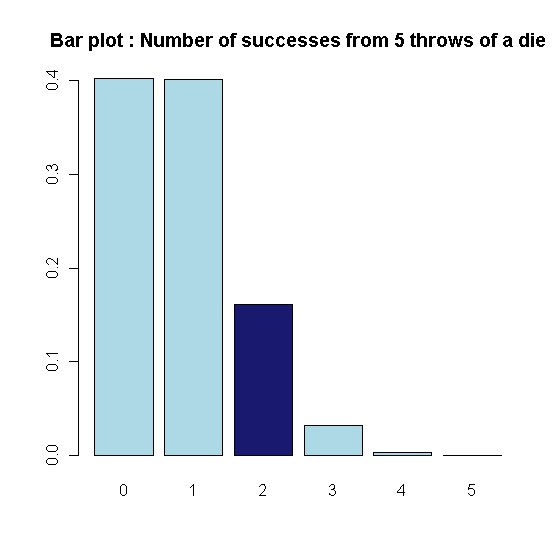
\includegraphics[scale=0.40]{3Bbarplot4}
\end{center}
}
%--------------------------------------------------------------------------------------%
\frame{
\frametitle{Binomial Probability}

\textbf{Remark} : The sum of the probabilities of each of the possible outcomes (i.e. no fours, one four etc) is equal to one.
\[P(X=0) + P(X = 1) + \ldots + P(X=5) = 1 \]

}
%--------------------------------------------------------%

\frame{
\frametitle{Binomial Example: At least two successes}

\begin{center}
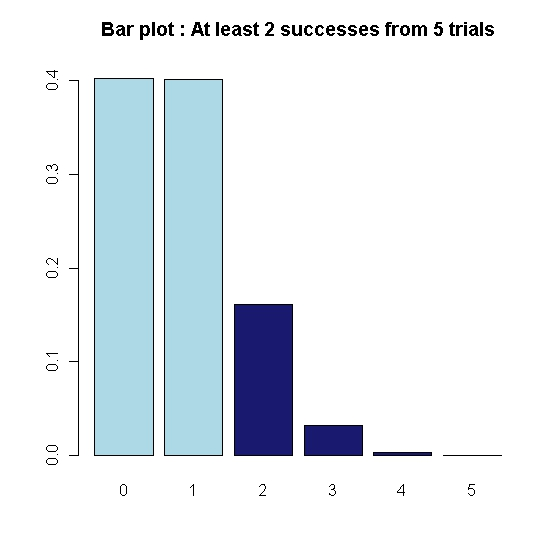
\includegraphics[scale=0.40]{3Bbarplot5}
\end{center}
}

%--------------------------------------------------------%

\frame{
\frametitle{Binomial Example: At least two successes}
\begin{itemize}
\item Suppose we were asked to find the probability of \textbf{\emph{at least}} 2 fours.
\item Can you suggest the most efficient way of computing this?
\item Suggestion: Compute $P(X=0)$ and $P(X = 1)$.
\item Together these probabilities are the complement probability of what we require.
\item $P(X \geq 2) = 1 - ( P(X=0) + P(X = 1))$.
\item (We will continue with this in future classes).
\end{itemize}
}
%--------------------------------------------------------------------------------------%
\frame{
\frametitle{Cumulative Distribution Function}


The cumulative distribution function (c.d.f.) of a discrete random variable $X$ is the function $F(t)$ which tells you the probability that X is less than or equal to t. \\ So if X has p.d.f. P(X = x), we have:

\[ F(t) = P(X \leq t) = \sum_{(i=0)}^{(i=t)} P(X = x) \]

In other words, for each value that X can be which is less than or equal to $t$, work out the probability that X is that value and add up all such results.

}




%--------------------------------------------------------%

\begin{frame}[fragile]
\frametitle{Binomial Example: Sample Problem}

Suppose there are twelve multiple choice questions in an English class quiz. Each question has five possible answers, and only one of them is correct. Find the probability of having four or less correct answers if a student attempts to answer every question at random.\\
\bigskip
\textbf{Solution:}
Since only one out of five possible answers is correct, the probability of answering a question correctly by random is $1/5=0.2$. We can find the probability of having exactly 4 correct answers by random attempts as follows.(Blackboard. Correct Answer is 13.29\%)
\begin{verbatim}
> dbinom(4, size=12, prob=0.2)
[1] 0.1329
\end{verbatim}
\end{frame}
%--------------------------------------------------------%




\end{document}


















\frame{
\frametitle{The Binomial Probability Distribution}
\begin{itemize}
\item The number of independent trials is denoted $n$.
\item The probability of a `success' is $p$
\item The expected number of `successes' from $n$ trials is $E(X) = np$
\end{itemize}
}
%---------------------------------------------------------------------------%
\frame{
\frametitle{Characteristics of a Poisson Experiment}
A Poisson experiment is a statistical experiment that has the following properties:
\begin{itemize}
\item The experiment results in outcomes that can be classified as successes or failures.
\item The average number of successes (m) that occurs in a specified region is known.
\item The probability that a success will occur is proportional to the size of the region.
\item The probability that a success will occur in an extremely small region is virtually zero.
\end{itemize}
Note that the specified region could take many forms. For instance, it could be a length, an area, a volume, a period of time, etc.
}

%---------------------------------------------------------------------------%
\frame{
\frametitle{Poisson Distribution}
A Poisson random variable is the number of successes that result from a Poisson experiment.

The probability distribution of a Poisson random variable is called a Poisson distribution.

Given the mean number of successes ($m$) that occur in a specified region, we can compute the Poisson probability based on the following formula:
}

%---------------------------------------------------------------------------%
\frame{
\frametitle{The Poisson Probability Distribution}
\begin{itemize}
\item The number of occurrences in a unit period (or space)
\item The expected number of occurrences is $m$
\end{itemize}
}

%---------------------------------------------------------------------------%
\frame{
\frametitle{Poisson Formulae}
The probability that there will be $k$ occurrences in a unit time period is denoted $P(X=k)$, and is computed as follows.
\Large
\[ P(X = k)=\frac{m^k e^{-m}}{k!} \]

}
%---------------------------------------------------------------------------%
\frame{
\frametitle{Poisson Formulae}
Given that there is on average 2 occurrences per hour, what is the probability of no occurences in the next hour? \\ i.e. Compute $P(X=0)$ given that $m=2$
\Large
\[ P(X = 0)=\frac{2^0 e^{-2}}{0!} \]
\normalsize
\begin{itemize}
\item $2^0$ = 1
\item $0!$ = 1
\end{itemize}
The equation reduces to
\[ P(X = 0)=e^{-2} = 0.1353\]
}
%---------------------------------------------------------------------------%
\frame{
\frametitle{Poisson Formulae}
What is the probability of one occurrences in the next hour? \\ i.e. Compute $P(X=1)$ given that $m=2$
\Large
\[ P(X = 1)=\frac{2^1 e^{-2}}{1!} \]
\normalsize
\begin{itemize}
\item $2^1$ = 2
\item $1!$ = 1
\end{itemize}
The equation reduces to
\[ P(X = 1) = 2 \times e^{-2} = 0.2706\]
}
%---------------------------------------------------------------------------%
\frame{
\frametitle{Continuous Random Variables}

\begin{itemize}
\item Probability Density Function
\item Cumulative Density Function
\end{itemize}


If X is a continuous random variable then we can say that the probability of obtaining a \textbf{precise} value $x$ is infinitely small, i.e. close to zero.

\[P(X=x) \approx 0 \]

Consequently, for continuous random variables (only),  $P(X \leq x)$ and $P(X < x)$ can be used interchangeably.

\[P(X \leq x) \approx P(X < x) \]


}

%---------------------------------------------------------------------------%
\frame{
\frametitle{Continuous Uniform Distribution}
A random variable X is called a continuous uniform random variable over the interval $(a,b)$ if it's probability density function is given by

\[ f_{X}(x)  =  { 1 \over b-a}   \hspace{2cm}  \mbox{ when } a \leq x \leq b\]

The corresponding cumulative density function is

\[ F_x(x) = { x-a \over b-a}   \hspace{2cm}  \mbox{ when } a \leq x \leq b\]

}

%-----------------------------------------------------------------------------%

\frame{

The mean of the continuous uniform distribution is

\[ E(X) = {a+b \over 2}\]

\[ V(X) = {(b-a)^2\over12}\]
}

%-----------------------------------------------------------------------------%

\frame{
\frametitle{The Memoryless property}
The most interesting property of the exponential distribution is the \textbf{\emph{memoryless}} property. By this , we mean that if  the lifetime of a component is exponentially distributed, then an item which has been in use for some time is a good as a brand new item with regards to the likelihood of failure.

The exponential distribution is the only distribution that has this property.
}

%--------------------------------------------------------%

\frame{
\frametitle{Random Variables}
A pair of dice is thrown. Let X denote the minimum of the two numbers which occur.
Find the distributions and expected value of X.
}
%-------------------------------------------------------------%
\frame{
\frametitle{Random Variables}
A fair coin is tossed four times.
Let X denote the longest string of heads.
Find the distribution and expectation of X.}
%-------------------------------------------------------------%
\frame{\frametitle{Random Variables}
A fair coin is tossed until a head or five tails occurs.
Find the expected number E of tosses of the coin.}
%-------------------------------------------------------------%
\frame{\frametitle{Random Variables}A coin is weighted so that P(H) = 0.75 and P(T ) = 0.25

The coin is tossed three times. Let X denote the number of
heads that appear.
\begin{itemize}
\item (a) Find the distribution f of X.
\item (b) Find the expectation E(X).
\end{itemize}
}

%-------------------------------------------------------------%
\frame{
\begin{itemize}
\item Now consider an experiment with only two outcomes. Independent repeated trials of such an experiment are
called Bernoulli trials, named after the Swiss mathematician Jacob Bernoulli (1654–1705). \item The term \textbf{\emph{independent
trials}} means that the outcome of any trial does not depend on the previous outcomes (such as tossing a coin).
\item We will call one of the outcomes the ``success" and the other outcome the ``failure".
\end{itemize}
}

%-------------------------------------------------------------%
\frame{
\begin{itemize}
 \item
Let $p$ denote the probability of success in a Bernoulli trial, and so $q = 1 - p$ is the probability of failure.
A binomial experiment consists of a fixed number of Bernoulli trials. \item A binomial experiment with $n$ trials and
probability $p$ of success will be denoted by
\[B(n, p)\]
\end{itemize}
}
%-------------------------------------------------------------%

%---------------------------------------------------------------------------%
\frame{
\frametitle{Probability Mass Function}
\begin{itemize} \item a probability mass function (pmf) is a function that gives the probability that a discrete random variable is exactly equal to some value. \item The probability mass function is often the primary means of defining a discrete probability distribution \end{itemize}
}
%------------------------------------------------------------------%
\frame{
Thirty-eight students took the test. The X-axis shows various intervals of scores (the interval labeled 35 includes any score from 32.5 to 37.5). The Y-axis shows the number of students scoring in the interval or below the interval.

\textbf{\emph{cumulative frequency distribution}}A  can show either the actual frequencies at or below each interval (as shown here) or the percentage of the scores at or below each interval. The plot can be a histogram as shown here or a polygon.
}




\end{document}



%---------------------------------------------------------------------------------------------------------------%
%----R Code ----
%---------------------------------------------------------------------------------------------------------------%
n=60000
Y=numeric(n)
for ( i in 1:n){

X=floor(runif(100,1,7))
Y[i]=sum(X)
}

Y
hist(Y,breaks=seq(300,400,by=10),main=c("Totals of 100 Die Throws"),cex.lab=1.4,font.lab=2,xlab=c("Total Score"))

hist(Y,breaks=seq(300,400,by=20),main=c("Totals of 100 Die Throws"),cex.lab=1.4,font.lab=2,xlab=c("Total Score"))



Z=seq(1:n)
Y/Z

plot(Y/Z,type="l",col="red",main=c("Die Rolls: Running Average"),font.lab=2,ylab="Average Value", xlab=
" Number of Throws")
abline(h=3.5,col="green")


#####################################################

plot(Z,Z.y,pch=16,col="red",ylim=c(2.5,5.5),main=c("Variance"),font.lab=2,ylab=" ", xlab="X: Green  Y: Blue  Z: Red" )

points(Y,Y.y,pch=16,col="blue" )
points(X,X.y,pch=16,col="green" )
points(c(1000,1000,1000),c(3,4,5),pch=18,cex=1.2)
lines(c(1000,1000),c(2.75,5.25),lty=3)



n=100000
Y=numeric(n)
for ( i in 1:n){

X=floor(runif(100,1,7))
Y[i]=mean(X)
}

Y
hist(Y,breaks=seq(270,430,by=2),main=c("Mean of 100 Die Throws (n= 100,000)"),cex.lab=1.4,font.lab=2,xlab=c("Mean of 100 throws")) 
